\documentclass[12pt,letter]{article}
\usepackage{mathptmx} % added for time new roman font
\usepackage[left=1in,right=1in,top=1in,bottom=1in]{geometry}
\usepackage[latin1]{inputenc}
\usepackage{amsmath}

% defines all example enviorment
\usepackage[framemethod=tikz]{mdframed} % added for the box around examples
\newtheorem{ex}{Example}
\numberwithin{ex}{section} % allows for the use of example numbers that lign up with the section numbers
\newenvironment{example}{\begin{mdframed}[middlelinewidth=0.5mm]\begin{ex}\normalfont}{\end{ex}\end{mdframed}}

% defines all review enviorment
\usepackage[framemethod=tikz]{mdframed} % added for the box around examples
\newtheorem{re}{Review}
\numberwithin{re}{section} % allows for the use of example numbers that lign up with the section numbers
\newenvironment{review}{\begin{mdframed}[middlelinewidth=2mm,roundcorner=20pt]\begin{re}\normalfont}{\end{re}\end{mdframed}}

% defines the quotation enviorment 
\usepackage{xcolor}
\newcommand{\quotebox}[2]{\begin{center}\fcolorbox{white}{blue!15!gray!15}{\begin{minipage}{0.9\linewidth}\vspace{10pt}\center\begin{minipage}{0.8\linewidth}{\space\Huge``}{#1}{\Huge''}{\break\null\hfill} {\small #2}  \end{minipage}\medbreak\end{minipage}}\end{center}}

% defines the definition enviorment 
\newcommand{\definitionbox}[2]{\begin{center}\fcolorbox{white}{blue!15!gray!15}{\begin{minipage}{0.9\linewidth}\vspace{10pt}\center\begin{minipage}{0.8\linewidth} {{\textbf{Definition} - }{#1}: {#2}}\end{minipage}\medbreak\end{minipage}}\end{center}}

\usepackage{amsfonts}
\usepackage{amssymb}
\usepackage{graphicx}
\usepackage{float}
\usepackage{booktabs}
%\usepackage{parskip} % remove all the paragraph indents

\usepackage{setspace}
%\usepackage[colorlinks=true]{hyperref}
\usepackage{textcomp} 
\usepackage{multicol} 


%%%%%%%		define the symbols for positive directions		%%%%%%
\makeatletter													%%	
																%%					
\newcommand*\curveplus{% positive counterclockwise				%%
  \mathbin{\rotatebox[origin=c]{90}{$\m@th\curvearrowleft$}+}}	%%
																%%
\newcommand*\rightplus{% positive right							%%
  \mathpalette\@rightplus\relax}								%%
\newcommand*\@rightplus[1]{%									%%
  \mathbin{\vcenter{\hbox{$\m@th\overset{#1+}{\to}$}}}}			%%
																%%	
\newcommand*\upplus{% positive up								%%
  \mathbin{+\mathord\uparrow}}									%%
																%%			
\newcommand*\downplus{% positive down							%%		
  \mathbin{+\mathord\downarrow}}								%%
  																%%		
\newcommand*\downrightplus{% positive down and right			%%	
  \mathbin{+ \rotatebox[origin=c]{-30}{$\m@th\rightarrow$}}}	%%
\makeatother 													%%	
%%%%%%%%%%%%%%%%%%%%%%%%%%%%%%%%%%%%%%%%%%%%%%%%%%%%%%%%%%%%%%%%%%


\usepackage{mathtools}          %loads amsmath as well added for the piece wise function
\DeclarePairedDelimiter\Floor\lfloor\rfloor
\DeclarePairedDelimiter\Ceil\lceil\rceil

 
\newcounter{NumberInTable}
\newcommand{\LTNUM}{\stepcounter{NumberInTable}{(\theNumberInTable)}}

\newcommand{\Laplace}[1]{\ensuremath{\mathcal{L}{\left[#1\right]}}}
\newcommand{\InvLap}[1]{\ensuremath{\mathcal{L}^{-1}{\left[#1\right]}}}
\renewcommand{\textuparrow}{$\uparrow$}


\begin{document}



\setcounter{section}{5}	
\section{Vibration Control}

Throughout this text we have studied various aspects related to analyzing and modeling vibrating systems. Therefore, it becomes prudent to look at methods for reducing or eliminating unwanted vibrations. However, before vibrations in a system can be effectively reduced they must be better understood in terms of their affects on the system understudy. For this reason, this chapter first introduces the vibration Nomograph, this is than followed by vibration isolation, absorption, and active suppression.  

\subsection{Vibration Nomograph}

There exist various methods and standards for measuring and describing acceptable levels of vibrations in systems, these include ISO/AWI 2631 for the evaluation of human exposure to whole-body vibrations and ISO 4866 for the measurement and effects of vibrations on structures. A common way to present the limits of a vibration is in a vibration nomograph.  A vibration nomograph is a simplified way to express the acceptable limits on a system while considering the displacement, velocity, acceleration and frequency of a system. A typical nomograph with various limits is presented in figure \ref{fig:Vibration_nomograph}. 

A vibration nomograph is a logarithmic plot that allows us to easily express the relationships between displacement, velocity, acceleration and frequency of a system. The vibration nomograph presented in figure \ref{fig:Vibration_nomograph} considers au undamped 1-DOF system system with a constant amplitude ($A$) experiencing harmonic motion that can be modeled as:
\begin{equation}
	x(t) = A \sin(\omega t)
\end{equation}
Therefore, the velocity and acceleration terms can be found by taking the derivatives of the displacement expression to yield:
\begin{equation}
	\dot{x}(t) = A \omega \cos(\omega t)
\end{equation}
and:
\begin{equation}
	\ddot{x}(t) = -A\omega^2 \sin(\omega t)
\end{equation}




\begin{figure}[H]
	\centering
	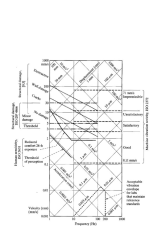
\includegraphics[]{../Figures/Vibration_nomograph.png}
	\caption{Vibration nomograph showing the acceptable limits of vibration for various applications. Adopted from \cite{Rao2017Mechanicalvibrations} and \cite{Macinante1984Seismicmountingsvibration}.}
	\label{fig:Vibration_nomograph}
\end{figure}







			\noindent
			

	\pagebreak
	\renewcommand{\thepage}{}
	\renewcommand\refname{References Cited}
	\pagestyle{plain}
	\bibliographystyle{unsrtDOI}
	\bibliography{Chapter_6_vibration_control}
	
\end{document}














